\begin{figure}[h!]
  \centering
  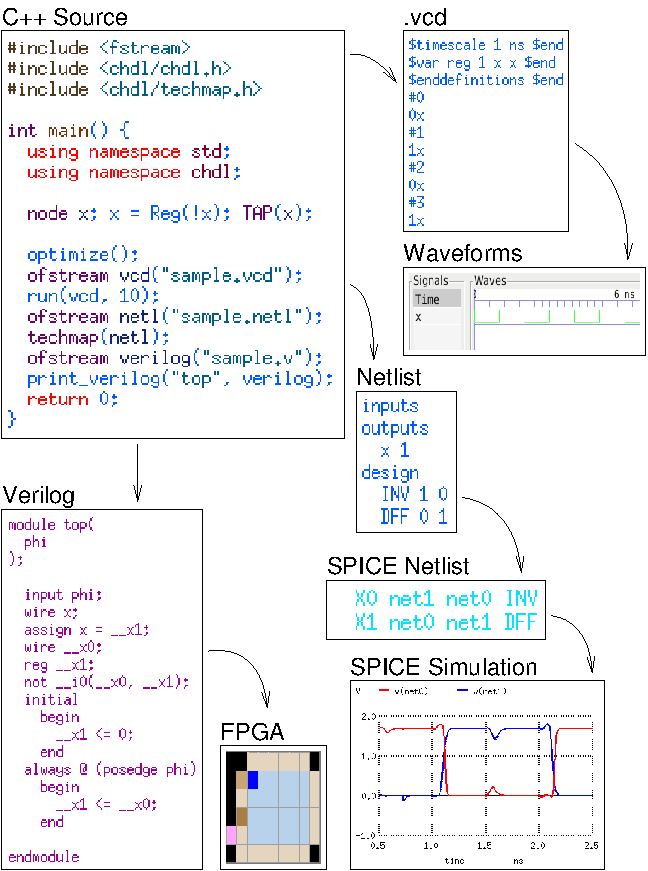
\includegraphics[width=3.5in]{fig/chdl}
  \caption{CHDL is a versatile \texttt{C++} hardware design library supporting a wide range of output formats.}
  \label{fig:chdl}
\end{figure}

An open source \texttt{C++}-based hardware design library called CHDL \cite{chdl} forms the core of the prototyping and gate-level simulation efforts.
CHDL designs are created by writing a high-level description in \texttt{C++}.
These descriptions can be incorporated into a program which, when compiled and run, produces any of a variety of outputs, which can include
\begin{itemize}
  \item Value Change Dump (\texttt{.vcd}) files representing simulation output.
  \item Optimized synthesizable Verilog source code.
  \item Intermediate netlists suitable for circuit-level simulation or place and route.
\end{itemize}
A very brief CHDL example is shown in Figure~\ref{fig:chdl} along with a variety of output formats.

Our ongoing effort to produce a heterogeneous architecture research prototype (HARP) has succeeded in producing a set of instruction set architectures collectively known as the HARP ISA, an assembler/linker/emulator tool, and a parameterized in-order, single-issue, register transfer level implementation called Harmonica.
The HARP ISA is parameterized fully predicated SIMD instruction set intended to be used in a wide range of processor designs.
Because of the parameterized nature of the HARP ISA and the Harmonica implementation thereof, it is versatile, being able to fill multiple roles in the so-called compute hierarchy.

Harmonica is a pipelined processor that issues instructions in-order and allows them to complete out-of-order.
It is built in a modular fashion so that functional units implementing various sets of instructions can be added or omitted as desired.
The minimum pipeline depth is four, but depending on the number of functional units installed and the number of outstanding instructions each might have, the total instructions in flight can be much higher.
Table~\ref{table:harp} provides an example of the range of core sizes and parameters possible with Harmonica.
These are on the small side, lacking floating point units and having relatively small register files.
In the figure, ``gates'' is the total post-optimization number of nand gates, D flip-flops, and inverters in the design.

\begin{table}
  \centering
  \begin{tabular}{ccc|cc}
    Bits&Regs&Lanes&  Gates& Crit. Path (Gates)\\
    \hline
    32  &   8&    1&  31811&           99\\
    32  &  16&    1&  36459&           99\\
    32  &  16&    2&  62295&           99\\
    32  &  16&    8& 217358&           99\\
    32  &  16&   16& 424117&           99\\
    64  &  16&    8& 544835&          105\\
    32  &  16&   32& 864220&           99\\
  \end{tabular}
  \caption{Harmonica implementation of HARP ISA with various parameters. All of these numbers represent integer-only cores with gshare branch prediction.}
  \label{table:harp}
\end{table}

This work does not exist in isolation from the higher-level simulation work.
Using a set of generic interface functions, a CHDL processor model has been demonstrated running within SST, using SST's MemHierarchy interface as its only memory system.
This integration will allow a seamless transition between high-level trace-driven models and low-level synthesizable hardware models and has the added advantage, since SST is a distributed simulation framework, of allowing multiple CHDL processor implementations to be simulated within SST in parallel.

The eventual goal of the HARP project is to run unmodified GPU kernels generated from the PTX intermediate form as well as non-SIMD benchmarks compiled from C.
For now, all of the applications are kernel benchmarks written directly in HARP assembly language.
